\begin{figure*}[t]
    %\vspace{-1.66em}
    \centering
    \hfill
    \subfloat[Runtime scaling with length ($d{=}4\%$, $r{=}1$)]
    {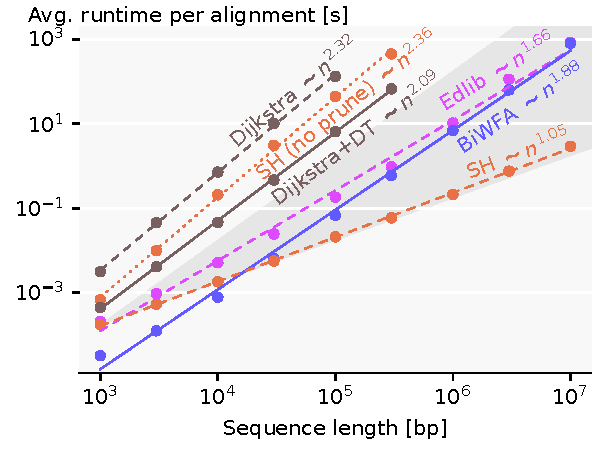
\includegraphics[scale=0.55]{plots/scaling_n.labels.pdf}\label{fig:scaling-n}}
    \hfill
    \subfloat[Runtime scaling with length ($d{=}12\%$, $r{=}2$)\!\!]
    {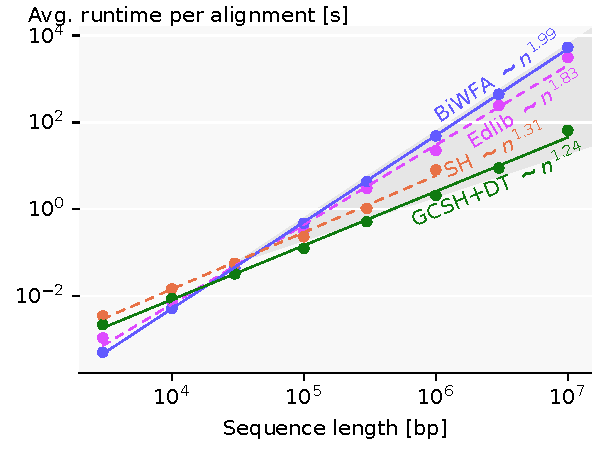
\includegraphics[scale=0.55]{plots/tools_e0.15_enlarged.labels.pdf}\label{fig:scaling-n-large}}
    \hfill
    \subfloat[Runtime scaling with divergence]
    {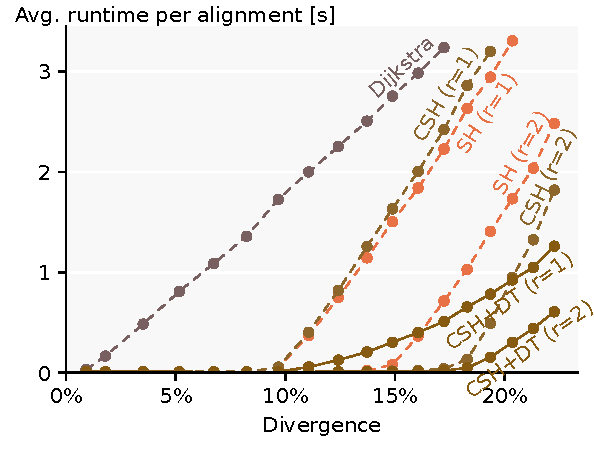
\includegraphics[scale=0.55]{plots/scaling_e.labels.pdf}\label{fig:scaling-e}}
    \hfill
    \caption{
      \textbf{Runtime comparison on synthetic data}
      \protect\subref{fig:scaling-n}\protect\subref{fig:scaling-n-large}
  Log-log plots comparing our simplest~(\SH) and most accurate
  heuristic~(\GCH with DT) to \edlib, \wfa, and other algorithms
      (averaged over $10^6$ to $10^7$ total bp, seed length $k{=}15$).
  The slopes of the bottom (top) of the dark-grey cones correspond to linear (quadratic) growth.
      \SH without
      pruning is dotted, and variants with DT are solid. At $4\%$ divergence,
      the complex techniques \CSH, \GCH, and DT (not shown) are as fast as \SH.
  Missing data points are due to exceeding the $\qty{32}{GiB}$ memory limit.
  \protect\subref{fig:scaling-e}
  Runtime scaling with divergence ($n{=}10^4$, $10^6$ total bp, $k{=}10$).
      \GCH (not shown) is as fast as \CSH.}
    \label{fig:synthetic}
\end{figure*}
